\documentclass{beamer}

\usepackage{amsfonts, amsmath, amssymb}
\usepackage{tikz}

\usetheme{Marburg}
\usecolortheme{orchid}
\usefonttheme{professionalfonts}


% Edit
\title{Insights from Discrete Mathematics \\ Integer Partitions}
\author{Ethan Li}
\date{May 11, 2024}  


\begin{document}

    % Title Page
    \begin{frame}
        \titlepage
    \end{frame}


    % Table of Contents
    \begin{frame}{Agenda}
        \tableofcontents
    \end{frame}


    \section{Introduction}
    % this is a slide
    \begin{frame}{Introduction}
        \begin{definition}
            A partition of a positive integer $n$ is written as a sum of positive integers. Different orders of the same partitions do not count as separate partitions
        \end{definition}

        \begin{example}
            Let $P(n)$ output the number of partitions for any number $n$.
            \begin{equation}
                P(0) = 1
            \end{equation}
            \begin{equation}
                P(1) = 1
            \end{equation}
            \begin{equation}
                P(4) = 5
            \end{equation}
            
            \scriptsize\centering\ $P(4)$ as $4$ can be written as $1$+$1$+$1$+$1$, $1$+$1$+$2$, $1$+$3$, $2$+$2$ and $4$
        \end{example}
    \end{frame}

    \section{Representations of the Partitions}
    % this is another slide
    \begin{frame}{Representations of the Partitions}{Ferrers diagram}
        \centering
        A partition can be represented graphically through \\ a Ferrers diagram
        \vspace{2em}
    
        \begin{minipage}[t]{0.48\textwidth}
            \centering
           {\tiny {$5$ = $2$+$2$+$1$ can be illustrated as follows:}}
            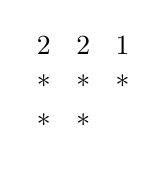
\begin{tikzpicture}[scale=0.5] 
                % Draw numbers
                \node at (1, 5) {$2$};
                \node at (2, 5) {$2$};
                \node at (3, 5) {$1$};

                % Draw stars corresponding to each number
                \foreach \x in {1,...,3}
                    \node at (\x, 4) {*};
                \foreach \x in {1,...,2}
                    \node at (\x, 3) {*};
            \end{tikzpicture}
        \end{minipage}\hfill
        \begin{minipage}[t]{0.48\textwidth}
            \centering
            {\tiny{If a partition's reverse is just itself, it's called self-conjugate.$10$ = ($4$, $3$, $2$, $1$) can be shown as: }}
                \vspace{2em}
                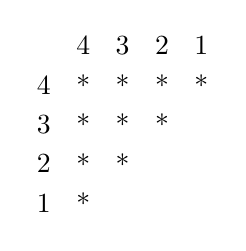
\begin{tikzpicture}[scale=0.5]
                    % Draw numbers
                    \node at (1, 5) {$4$};
                    \node at (2, 5) {$3$};
                    \node at (3, 5) {$2$};
                    \node at (4, 5) {$1$};
                    \node at (0, 4) {$4$};
                    \node at (0, 3) {$3$};
                    \node at (0, 2) {$2$};
                    \node at (0, 1) {$1$};
                
                    % Draw stars corresponding to each number
                    \foreach \x in {1,...,4}
                        \node at (\x, 4) {*};
                    \foreach \x in {1,...,3}
                        \node at (\x, 3) {*};
                    \foreach \x in {1,...,2}
                        \node at (\x, 2) {*};
                    \node at (1, 1) {*};
                \end{tikzpicture}
        \end{minipage}
    \end{frame}
    
    % this is another slide
    \begin{frame}{Representations of the Partitions}{Young Diagram}
        \href{https://youtu.be/8qc71j8yhG0}{\small\ Click here for animation demo using Python Manim} \\
        \begin{figure}\
        \centering
            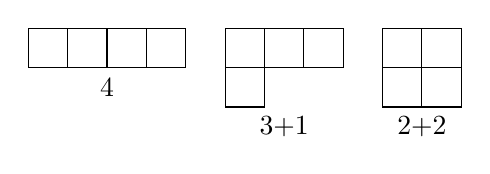
\begin{tikzpicture}[scale=0.5]
                % Partition 4
                \draw (0,0) rectangle (4,1);
                \draw (1,0) -- (1,1);
                \draw (2,0) -- (2,1);
                \draw (3,0) -- (3,1);
                \node at (2, -0.5) {$4$};
            
                % Partition 3+1
                \draw (5,0) rectangle (8,1);
                \draw (6,0) -- (6,1);
                \draw (7,0) -- (7,1);
                \draw (5,0) rectangle (6,-1);
                \node at (6.5, -1.5) {$3$+$1$};

                % Partition 2+2
                \draw (9,0) rectangle (11,1);
                \draw (9,0) rectangle (11,-1);
                \draw (10,0) -- (10,1);
                \draw (10,-1) -- (10,0);
                \node at (10, -1.5) {$2$+$2$};
            \end{tikzpicture}
        \end{figure}
        \begin{figure}[h]
        \centering
            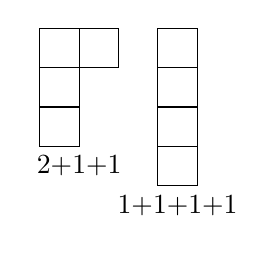
\begin{tikzpicture}[scale=0.5]
                % Partition 2+1+1
                \draw (0,-4) rectangle (2,-3); % Shifted to start at (0, -4)
                \draw (1,-4) -- (1,-3);
                \draw (0,-4) rectangle (1,-5);
                \draw (0,-5) rectangle (1,-6);
                \node at (1, -6.5) {$2$+$1$+$1$};
            
                % Partition 1+1+1+1
                \draw (3,-4) rectangle (4,-3); % Shifted to start at (3, -4)
                \draw (3,-4) rectangle (4,-5);
                \draw (3,-5) rectangle (4,-6);
                \draw (3,-6) rectangle (4,-7);
                \node at (3.5, -7.5) {$1$+$1$+$1$+$1$};
            \end{tikzpicture}
            \caption{Young diagram for all partitions of $4$}
        \end{figure}
    \end{frame}


    \section{Euler’s Generating Functions}
    % this is a slide
    \begin{frame}{Euler’s Generating Functions}
        \begin{equation}
            \sum_{n=0}^{\infty} p(n) x^n = \frac{1}{\prod_{p=1}^{\infty} (1-x^p)}, \quad \text{where } |x| < 1
        \end{equation}

        \begin{example}
            To find the number of partitions of $7$, we examine the coefficient of $x^7$:
            \begin{equation}
                (1 + x^{1\cdot(1)} + x^{1\cdot(2)} + x^{1\cdot(3)} + \ldots )(1 + x^{2\cdot(1)} + x^{2\cdot(2)} + x^{2\cdot(3)} + \ldots ) \ldots
            \end{equation} \\
            Expanding above to get
            \begin{equation}
                1 + x + 2x^2 + 3x^3 + 5x^4 + 7x^5 + 11x^6 + 15x^7 + 22x^8 + \ldots
            \end{equation}
            \begin{equation}
                P(7) = 15
            \end{equation}
        \end{example}
    \end{frame}

    \section{The Coins Change Problem}
    % this is a slide
    \begin{frame}{The Coins Change Problem}{How many ways to change $\$1$ ?}
        \begin{figure}[h!]
        \centering
            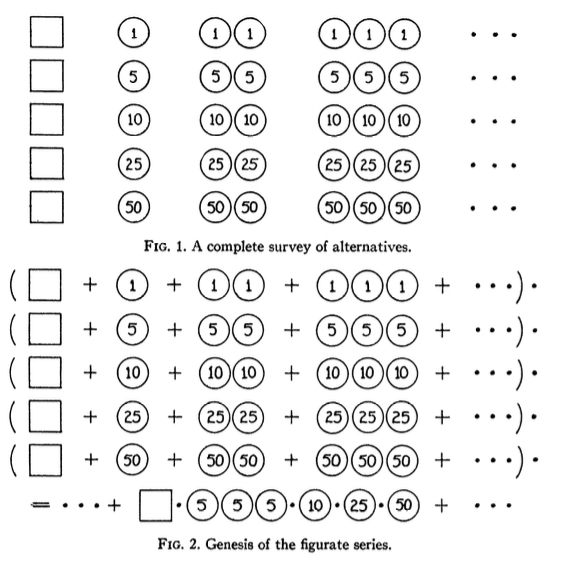
\includegraphics[width=6cm]{images/coins-change.jpg}
            \caption{\href{https://youtu.be/PmR1eRswj3A}{\small\ Click here for animation demo using Python Manim}}
        \end{figure}
    \end{frame}

    % this is a slide
    \begin{frame}{The Coins Change Problem}{Using the Coins Change problem to derive the Euler’s Generating Function}
        \begin{definition}
            Interpret the coins change problem in mathematical form as follows:
            \begin{center}{Let \( P_n \) denote the number of ways of paying \(n\) cents \\ with cents, nickels, dimes, quarters, and half dollars.\\ Given \(P_4=1\), \(P_6=2\), and \(P_{10}=4\), what is \(P_{100}\) ?}
            \end{center}
        \end{definition}
        \begin{proof}
            Please visit \href {https://github.com/ethan201not404/Math-Mentorship-2024/blob/main/2024MathMentorshipByEthanLi.pdf}{the section $2.2$ of my research paper available on the GitHub (link) for complete derivation for Euler's Generating Function based on the coins change problem.}
        \end{proof}
    \end{frame}

    \section{Hardy-Ramanujan’s Asymptotic Expression}
    % this is a slide
    \begin{frame}{Hardy-Ramanujan’s Asymptotic Expression}
        \begin{definition}
            Godfrey Hardy and Srinivasa Ramanujan create an asymptotic formula for partitioning a number \(n\) using the circle method and modular functions
        \end{definition}
        \begin{equation}
            p(n) \approx \frac{1}{4n\sqrt{3}} e^{\pi \sqrt{\frac{2n}{3}}} \quad \text{as} \quad n \to \infty
        \end{equation} \\

        \centering \href{https://youtu.be/UYjqhT5xnsY}{Click here for animations demo using Python Manim}\
    \end{frame}

\end{document}
